La primera solución planteada para el abastecimiento de energía de la UBM se basa en la transferencia de energía al dispositivo del ave por medio de radiación electromagnética. A continuación se detalla el análisis de factibilidad tecnológica realizado y las conclusiones tomadas de esta propuesta.

\Subsubsubsection{Planteamiento del Problema}

La morfología del nido plantea la necesidad de recargar la UBM a distancias de entre 32 y 64 cm. Esto es dictado por las mínimas y máximas dimensiones medidas del nido entre la bóveda, donde se puede colocar electrónica, y el fondo, donde duerme el ave \cite{ref:PaperValeriaOjeda}.

En el mejor de los casos, el pájaro carpintero permanece por ocho horas en el nido mientras duerme, y luego cuida a las crías turnándose con la hembra durante el día. Por lo tanto, este permanecería un total de aproximadamente doce horas en el nido.

En el peor de los casos, el ave únicamente permanece seis horas dentro del nido para dormir.

Como la UBM tiene un consumo diario de

\begin{equation}
2.5 \ V \cdot 1 \ mA \cdot 24 \ hs = 60 \ mWh
\end{equation}

por lo que, tomando ambos casos, se obtiene un requerimiento de transmisión de potencia de

\begin{equation}
	\begin{cases} 
       \frac{60 \ mWh}{11 \ hs}= 5.5 \ mW & \text{Mejor caso} \\
       \frac{60 \ mWh}{8.5 \ hs} = 7 \ mW & \text{Peor caso}    
    \end{cases}
\end{equation}

\Subsubsubsection{Carga por Acoplamiento Magnético}

La transmisión inalámbrica de potencia por acoplamiento magnético se basa en generar un campo magnético al hacer circular corriente por un arreglo de bobinas gracias a la Ley de Ampere.

\begin{equation}
\nabla \times \mathbf{B} = \mu_0\left( \mathbf{J} + \epsilon_0 \frac{\partial \mathbf{B}}{\partial t} \right)
\end{equation}

Este campo magnético es captado por una o más bobinas receptoras las cuales generan a causa de este una fuerza electromotriz según la Ley de Faraday. 

\begin{equation}
\nabla \times \mathbf{E} = -\frac{\partial \mathbf{B}}{\partial t}
\end{equation}

De esta manera, se genera un sistema que actúa como transformador, utilizando como reluctancia al aire que separa ambas bobinas, con un factor de acople $k$ definido como

\begin{equation}
k = \frac{M}{\sqrt{L_1L_2}}
\end{equation}

donde $M$ es el coeficiente de mutua-inductancia entre las bobinas y $L_1$ y $L_2$ las auto-inductancias de las bobinas. 

La eficiencia en la transmisión de energía de este método es alta \cite{ref:wpteff}, pero depende en gran medida por el factor de acople entre ambas bobinas. Este factor de acople disminuye considerablemente con la distancia y la desalineación entre bobinas \cite{ref:wirelesschargingkeyelements} \cite{ref:couplingfactor_1}.

Como las distancias a las que la transmisión se debe efectuar son de entre 32 y 64 cm y no se puede garantizar alineación entre bobinas al estar sujeto al comportamiento impredecible del ave, se descarta este método como solución.

\Subsubsubsection{Carga por Radiofrecuencia}

Si se parte de la ecuación del campo magnético en el eje azimutal de un dipolo de hertz, se tiene que
\begin{equation}
E_\theta = -\frac{\eta}{4\pi}I \cdot \Delta L \cdot k^2 \cdot sin\theta \cdot e^{-jkr} \left[ \frac{1}{jkr}+\left( \frac{1}{jkr}\right)^2 + \left(\frac{1}{jkr}\right)^3 \right]
\end{equation}
donde los últimos tres términos se denominan, en orden de aparición, término de campo lejano, campo cercano radiativo, y campo cercano reactivo. 

Las fronteras entre estos campos no están estrictamente fijadas, ya que varían con el tipo y tamaño de antena. Para el caso de antenas eléctricamente cortas, es decir, más cortas que media longitud de onda, se adopta el siguiente criterio

\begin{equation}
\begin{cases} 
          0 < d <\frac{\lambda}{2\pi} & \text{Campo cercano reactivo o inductivo} \\
          \frac{\lambda}{2\pi} < d \overset{\approx}{<} \lambda & \text{Campo cercano radiativo o de Fresnel} \\
          \lambda \overset{\approx}{<} d \overset{\approx}{<} 2\lambda & \text{Zona de transición} \\
          2\lambda \overset{\approx}{<} d < \infty  & \text{Campo lejano o de Fraunhofer} 
       \end{cases}
\end{equation}

La zona de campo cercano puede dividirse entre la zona reactiva-inductiva y la zona radiativa o de Fresnel. 

En la zona reactiva la relación entre los campos eléctricos y magnéticos no es predecible. Además, como no solo hay ondas electromagnéticas siendo irradiadas en esta zona, sino que también hay una cierta cantidad de energía siendo almacenada en la cercanía de la antena, la verdadera densidad de potencia se torna difícil de encontrar.

En el caso de la zona radiativa o de Fresnel, toda la energía es radiada. Sin embargo, la relación entre el campo eléctrico y magnético sigue siendo impredecible.

A una distancia entre una y dos longitudes de onda, los efectos de campo cercano comienzan a cesar, mientras que los efectos de campo lejano comienzan a aparecer. Es en esta zona por lo tanto, que ambos efectos están presentes y tienen importancia \cite{ref:NearFieldVsFarField}. Los dispositivos RFID suelen operar en esta zona \cite{ref:NearFieldUHFRFID}.

Por otro lado, el campo lejano es el utilizado para realizar todo tipo de telecomunicaciones hoy en día. En esta zona, el campo eléctrico y campo magnético son ortogonales y la razón entre ambos es la impedancia del medio. Además, el vector de Poynting, definido como $\vec{S} = \vec{E}\times \vec{H}$, provee una medida de la energía electromagnética radiada \cite{ref:PhysicsOscillations}.

Para analizar la potencia recibida en la antena receptora, la cual estará montada en la mochila, se realiza el balance de potencias del circuito electromagnético, por lo que partiendo de la ecuación de transmisión de Friis, se tiene que

\begin{equation}
\frac{P_r}{P_t} = \left( \frac{A_rA_r}{d^2\lambda ^2} \right)
\end{equation}
reescribiendo esta fórmula para utilizar las ganancias de las antenas en vez de las áreas efectivas, e incluyendo otras pérdidas del circuito electromagnético, se arriba a

\begin{equation}
P_r[dBm] = P_t[dBm] + Gt[dB] + G_r[dB] - L_{bf}[dB] - L_{cab}[dB] - L_{roe}[dB] - L_{r}[dB]
\end{equation}
donde $P_r$ es la potencia recibida en la antena receptora, $P_t$ la potencia emitida por la antena transmisora, $G_t$ la ganancia de la antena transmisora, $G_r$ la ganancia de la antena receptora, $L_{bf}$ las pérdidas por espacio libre, $L_{cab}$ las pérdidas en los cables de ambas antenas, $L_{roe}$ las pérdidas por retorno en ambas antenas, y $L_{r}$ las pérdidas por desacople entre las líneas de transmisión y las antenas.

Para el caso de la pérdida por espacio libre, esta se puede calcular como

\begin{equation}
L_{bf} = 32.5dB + 20log_{10}f[MHz]+20log_{10}R[km]
\end{equation}
mientras que el resto de los datos se puede obtener por medio de las hojas de datos o ensayos de las antenas, exceptuando la potencia a ser calculada y las pérdidas por desacople, las cuales dependen constructivamente del diseño de la líneas de transmisión que conectan con las antenas.

\Subsubsubsection{Banda de Frecuencia Adoptada}

Se puede observar que las pérdidas de espacio libre aumentan mediante crece la frecuencia de la onda electromagnética emitida. Esto plantea una situación de compromiso. Si la frecuencia es muy alta, las pérdidas por espacio libre serán muy grandes. Mientras que si la frecuencia es muy baja, la longitud de onda será muy grande, por lo que se estaría trabajando en el campo reactivo. Esto no es deseado debido a la imposibilidad de determinar con precisión la densidad de potencia.

Se decidió utilizar la banda de 915 MHz por las siguientes razones:
\begin{itemize}
\item La zona de transición ocurre entre 32.8 y 65.6 cm que concuerda con las distancias mínimas y máximas entre emisor y receptor. Si bien no estaremos trabajando en campo lejano, esto no acarrea problemas, ya que hay basta cantidad de antecedentes del uso de los efectos de campo cercano en dispositivos comerciales \cite{ref:NearFieldUHFRFID} \cite{ref:Humavox}.
\item Esta frecuencia pertenece a la banda ISM, la cual está reservada para propósitos industriales, científicos o médicos, excluyendo las aplicaciones de telecomunicaciones \cite{ref:ITUISM}, atribuidas a la Región 2 definida por la ITU como América \cite{ref:ITUREGION}.
\end{itemize}
 
\Subsubsubsection{Condiciones de Borde}

Para realizar las comparaciones entre antenas transmisoras, se tuvieron en cuenta los siguientes criterios:
\begin{itemize}
\item \textbf{Dimensiones:} La antena transmisora deberá ser colocada en la bóveda del nido, dado que ese es el único lugar donde se puede colocar electrónica sin que esta sea perturbada por las aves y vice versa. El volumen de la bóveda se puede aproximar a el de un cilindro macizo chato de diámetro entre 7.9 y 9.7 cm y aproximadamente 5 cm de altura, por lo que las dimensiones de la antena emisora estarán acotadas por estos valores.
\item \textbf{Directividad:} Se quiere que la potencia enviada a la antena se transforme en radiación electromagnética que llegue a la mochila del ave, por lo que radiación que no sea dirigida directamente hacia el fondo del nido será potencia desperdiciada. Es por esto que se quiere una alta directividad en la antena emisora. También hay un límite máximo en la directividad de la antena. Sin embargo, esta limitación no se alcanzará, dado que la tecnología a utilizar será de antenas del tipo planas, más cortas eléctricamente que media longitud de onda por cuestiones de limitaciones en las dimensiones. 
\item \textbf{Potencia Máxima:} Como las pérdidas en el circuito electromagnético son grandes, una muy baja parte de la potencia enviada a la antena transmisora formará parte de la potencia entregada a las baterías de la mochila, por lo que para recibir la potencia necesaria, se debe transmitir en el orden de los watts. Es por esto que la potencia máxima es una especificación relevante al momento de decidir entre soluciones.
\end{itemize}

Mientras que para el caso de las antenas receptoras, se tuvieron en cuenta los siguientes criterios:
\begin{itemize}
\item \textbf{Eficiencia:} Esta será la especificación más importante y es la que determinará la factibilidad de la solución. Se buscará la mayor eficiencia posible para lograr transmitir a las baterías la potencia recibida por el campo electromagnético.
\item \textbf{Lóbulo isotrópico:} Como se desconoce cuál será la posición del ave dentro del nido, se requiere que el lóbulo de radiación de la antena receptora sea lo más isotrópico posible, garantizando una recepción de potencia uniforme sin importar la posición del ave. Se buscará una ganancia menor a 2 dBi.
\item \textbf{Peso:} El ave no puede cargar con más de un cierto porcentaje de su propio peso, por lo que minimizar esta especificación es crucial.
\item \textbf{Dimensiones:} Es necesario no perturbar al ave con la mochila. Esto requiere que la antena receptora posea las mínimas dimensiones posibles. Sin embargo, como la banda a utilizar será la de 915 MHz y un cuarto de onda en esta frecuencia es alrededor de 8 cm, existe una relación de compromiso entre las dimensiones de la antena receptora y la eficiencia de esta.
\end{itemize}

Finalmente, una restricción a tener en cuenta para ambas antenas será el costo.

\Subsubsubsection{Cargador}

El bloque del cargador de la UBM consiste en un receptor y un transmisor de potencia. La transmisión inalámbrica consta, por el lado del transmisor, de un oscilador HM-TRPW-RS232 de $915 \ MHz$ el cual está comandado por la R-Pi y se comunica mediante UART; como así también de un amplificador de potencia de $3 \ W$ máximos alimentado por una etapa DC-DC Xl6009 de $12 \ V$ a $15 \ V$.

Por el lado del receptor, se encuentra el integrado P1110B, el cual almacena energía temporalmente en un capacitor para realizar posteriormente la carga de la UBM.

\begin{figure}[H]
	\centering	
	\includegraphics[width=0.9\textwidth, page=8]{ImagenesIngenieria de Detalle/FlowChart.pdf}
	\caption{Diagrama en bloques cargador.}
	\label{fig:diagrama_hardware_antenas}
\end{figure}

Para la transmisión de la señal de $915 \ MHz$ se utilizará cable del tipo \textit{RG-213} el cual posee bajas pérdidas de $23.054 \ \nicefrac{dB}{100m}$.\\

\textbf{Oscilador 915 MHz}

\begin{figure}[H]
	\centering	
	\includegraphics[width=0.5\textwidth, page=8]{ImagenesIngenieria de Detalle/hmtrpwrs232}
	\caption{Módulo utilizado como oscilador HM-TRPW-RS232.}
	\label{fig:oscilador}
\end{figure}

Debido a la falta de stock mundial de componentes electrónicos a causa de la pandemia, se utilizó un módulo transciever FSK que opera en la banda de 915MHz. Este módulo HM-TRPW-RS232 puede generar la señal carrier de hasta $20 \ dBm$ y posee interfaz RS-232 para la comunicación UART.

\begin{itemize}
	\item Potencia máxima de $20 \ dBm$.
	\item Alimentación $100 \ mA@20 \ dBm$.
	\item Corriente suspendido $1 \ \mu A$.
	\item Velocidad de comunicación $1.2 \ kbps - 115.2 \ kbps$.
	\item Dimensiones $44.1 \times 30  \times 1.2 \ mm$.
\end{itemize}

\textbf{Amplificador de Potencia}

Para el amplificador de potencia de RF, como las unidades a producir serán muy pocas, no se justifican las horas necesarias para diseñar el circuito y la placa impresa de un amplificador de RF. Por esta razón, se utilizará uno comercial. 

\textbf{DC-DC}

\tbc

\textbf{P1110B}

\begin{figure}[H]
	\centering	
	\includegraphics[width=0.5\textwidth, page=8]{ImagenesIngenieria de Detalle/p1110b}
	\caption{Módulo utilizado como power harvester.}
	\label{fig:p1110b}
\end{figure}

Para la recepción de la radiofrecuencia se utilizará el power harvester P1110B. Este integrado toma la señal de radiofrecuencia y realiza con esta la carga de un capacitor. Cuando el capacitor llega a un valor de tensión máximo, habilita la salida mediante una etapa DC-DC hasta que el capacitor baja su tensión por debajo de un mínimo para volver a cargarse hasta el máximo.


\begin{itemize}
\item Eficiencia del $70 \ \%$.
\item Adaptado internamente a $50 \ \Omega$.
\item Operación por encima de $-5 \ dBm$.
\item Opción de carga para Li-ion y baterías alcalinas.
\end{itemize}

\Subsubsubsection{Amplificador de Potencia}

Para el amplificador de potencia se tuvieron en cuenta distintos módulos armados.

\begin{table}[H]
\centering
\begin{tabular}{|c|c|c|c|c|}
\hline
\textbf{\begin{tabular}[c]{@{}c@{}}Aspectos\\ comparativos\end{tabular}}         & \textbf{\begin{tabular}[c]{@{}c@{}}\href{https://www.ebay.com/itm/133414335638}{NWDZ RF PA}\\ \href{https://www.ebay.com/itm/133414335638}{V2.0}\end{tabular}} & \textbf{\begin{tabular}[c]{@{}c@{}}\href{https://www.ebay.com/itm/284470793842}{Unbranded Broadband}\\ \href{https://www.ebay.com/itm/284470793842}{RF Amplifier}\end{tabular}} & \textbf{\begin{tabular}[c]{@{}c@{}}\href{https://www.ebay.com/itm/124120749418}{DH-RF}\\ \href{https://www.ebay.com/itm/124120749418}{V2017}\end{tabular}} & \textbf{\begin{tabular}[c]{@{}c@{}}\href{https://www.ebay.com/itm/283538071937}{JP-2Y560895}\\ \href{https://www.ebay.com/itm/283538071937}{RF Amplifier}\end{tabular}} \\ \hline
\textbf{Costo [USD]}                                                             & 18.59                                                                                                                                                                                                                                               & 9.82                                                                                                                                                                                                                                                  & 23                                                                                                                                                                                                              & 69.31                                                                                                                                                                                                                            \\ \hline
\textbf{Alimentación [V]}                                                        & 12-15                                                                                                                                                                                                                                               & 12                                                                                                                                                                                                                                                    & 15                                                                                                                                                                                                              & 24-28                                                                                                                                                                                                                            \\ \hline
\textbf{Frecuencia [MHz]}                                                        & 2-700                                                                                                                                                                                                                                               & 1-930                                                                                                                                                                                                                                                 & 1-1000                                                                                                                                                                                                          & 915 +- 25                                                                                                                                                                                                                        \\ \hline
\textbf{\begin{tabular}[c]{@{}c@{}}Potencia salida\\ máxima [dBm]\end{tabular}}  & 34.8                                                                                                                                                                                                                                                & 29                                                                                                                                                                                                                                                    & 35                                                                                                                                                                                                              & 42                                                                                                                                                                                                                               \\ \hline
\textbf{\begin{tabular}[c]{@{}c@{}}Potencia entrada\\ máxima [dBm]\end{tabular}} & 10                                                                                                                                                                                                                                                  & 0                                                                                                                                                                                                                                                     & 0                                                                                                                                                                                                               & 23                                                                                                                                                                                                                               \\ \hline
\textbf{\begin{tabular}[c]{@{}c@{}}Ganancia de\\ potencia [dB]\end{tabular}}     & 35                                                                                                                                                                                                                                                  & 29                                                                                                                                                                                                                                                    & 32                                                                                                                                                                                                              & Ajustable                                                                                                                                                                                                                        \\ \hline
\textbf{Dimensiones [cm]}                                                        & 7x3                                                                                                                                                                                                                                                 & 5x5                                                                                                                                                                                                                                                   & 3.7x5.6                                                                                                                                                                                                         & 4x8                                                                                                                                                                                                                              \\ \hline
\textbf{Imagen}                                                                  & \includeintable{.1}{ImagenesIngenieria de Detalle/nwdz}                                                                                                                                                                                             & \includeintable{.1}{ImagenesIngenieria de Detalle/unbranded}                                                                                                                                                                                          & \includeintable{.1}{ImagenesIngenieria de Detalle/DH-RF-V2017}                                                                                                                                                  & \includeintable{.1}{ImagenesIngenieria de Detalle/s-l1600}                                                                                                                                                                       \\ \hline
\end{tabular}
\end{table}

\Subsubsubsection{Integrado de Energy Harvesting}

Se investigaron diversos métodos de transmisión de energía inalámbrica a través de campos electromagnéticos. Dentro de estos se en cuenta el campo cercano y el de radiofrecuencia. El primero se caracteriza por ser puramente imaginario y por poseer una caída proporcional al cuadrado de la distancia, mientras que el segundo (radiación) cae linealmente.

Debido a que la aplicación es de una distancia que cae en el rango del campo lejano, se optó por la radiofrecuencia. Es así que surgieron los integrados IC-P2110 y IC-P1110 de PowerCast, los cuales permiten la recolección de energía de radio frecuencia almacenando esta en capacitores o con la opción de directamente cargar una batería (P1110). A continuación se comparan los dos IC.

\begin{table}[H]
\centering
\begin{tabular}{|c|c|c|}
\hline
\textbf{\begin{tabular}[c]{@{}c@{}}Aspectos\\ comparativos\end{tabular}}                          	&  \textbf{\href{https://www.powercastco.com/documentation/p1110-evb-datasheet/}{IC-P1110}}  	&\textbf{\href{https://www.powercastco.com/wp-content/uploads/2016/12/P2110B-Datasheet-Rev-3.pdf}{IC-P2110}}                 \\ \hline
\textbf{Costo [USD]}                                                                              	& 48.33	                                                                                           				& 32                                                                                              		\\ \hline
\textbf{\begin{tabular}[c]{@{}c@{}}Funcionalidad\\ principal\end{tabular}}                          & \begin{tabular}[c]{@{}c@{}}Recolección y almacenamiento\\ de energía para uso variado\end{tabular} 			& \begin{tabular}[c]{@{}c@{}}Recolección de energía para carga\\ de baterías/Capacitores\end{tabular} 	\\ \hline
\textbf{\begin{tabular}[c]{@{}c@{}}Frecuencia de\\ trabajo [MHz]\end{tabular}}                    	& 910 $\sim$ 928                                                                                     			& 910 $\sim$ 928                                                                                        \\ \hline
\textbf{\begin{tabular}[c]{@{}c@{}}Eficiencia del PH\\ para RFin = 11 dBm\end{tabular}}            	& 60 \%                                                                                               			& 45 \%                                                                                                 \\ \hline
\textbf{\begin{tabular}[c]{@{}c@{}}Corriente de salida\\ para RFin = 11 dBm\end{tabular}}           & 3 mA                                                                                                			& -                                                                                                     \\ \hline
\textbf{\begin{tabular}[c]{@{}c@{}}Timepo de carga \\ inicial del capacitor [s]\end{tabular}} 	  	& -                                                                                                   			& < 5                                                                                           		\\ \hline
\textbf{\begin{tabular}[c]{@{}c@{}}Posee placa\\ de evaluación\end{tabular}}                  		& Sí                                                                                                  			& Sí                                                                                                    \\ \hline
\textbf{\begin{tabular}[c]{@{}c@{}}Impedancia de\\ entrada  [$\Omega$] \end{tabular}}             	& 50                                                                                                  			& 50                                                                                                    \\ \hline
\textbf{\begin{tabular}[c]{@{}c@{}}Temperatura de\\ operación [°C]\end{tabular}}                  	& -40 $\sim$ 85                                                                                       			& -40 $\sim$ 85                                                                                         \\ \hline
\end{tabular}
\caption{Comparación entre cargadores.}
\end{table}

\Subsubsubsection{Comparación entre Antenas}
\begin{table}[H]
\centering
\begin{tabular}{|c|c|c|c|}
\hline
\textbf{\begin{tabular}[c]{@{}c@{}}Aspectos\\ comparativos\end{tabular}}    & \textbf{\href{https://abracon.com/patchantenna/APAE915R2540ABDB1-T.pdf}{APAE915R2540ABDB1-T}} & \textbf{\href{https://www.digikey.com/en/products/detail/pulselarsen-antennas/W3215/9838686}{W3215}} & \textbf{\href{https://cdn.taoglas.com/datasheets/ISPC.91A.09.0092E.pdf}{ISPC.91A.09.0092E}} \\ \hline
\textbf{Costo [USD]}                                                        & 3.66                                                                                 & 12.47                                                                                       & 20.91                                                                              \\ \hline
\textbf{Dimensiones [mm]}                                                   & 25 x 25 x 4                                                                          & 40 x 40 x 6                                                                                 & 47 x 47 x 6.5                                                                      \\ \hline
\textbf{\begin{tabular}[c]{@{}c@{}}Frecuencia\\ Central [MHz]\end{tabular}} & 915                                                                                  & 915                                                                                         & 915                                                                                \\ \hline
\textbf{Impedancia [$\Omega$]}                                              & 50                                                                                   & 50                                                                                          & 50                                                                                 \\ \hline
\textbf{Polarización}                                                       & RHCP                                                                                 & Lineal vertical                                                                             & RHCP                                                                               \\ \hline
\textbf{Ganancia [dBi]}                                                     & 1.5                                                                                  & 4.5                                                                                         & 5 (30 x 30 ground plane)                                                           \\ \hline
\textbf{ROE}                                                                & 1.5                                                                                  & 1.23                                                                                        & 1.28                                                                               \\ \hline
\textbf{Imagen}                                                             & \includeintable{.1}{ImagenesFactibilidad/ANT1}                                       & \includeintable{.1}{ImagenesFactibilidad/ANT2}                                              & \includeintable{.1}{ImagenesFactibilidad/ANT3}                                     \\ \hline
\textbf{Lóbulo}                                                             & \includeintable{.1}{ImagenesFactibilidad/LOB1}                                       & \includeintable{.1}{ImagenesFactibilidad/LOB2}                                              & \includeintable{.1}{ImagenesFactibilidad/LOB3}                                     \\ \hline
\end{tabular}
\caption{Comparación entre antenas transmisoras (Parte 1).}
\end{table}

\begin{table}[H]
\centering
\begin{tabular}{|c|c|c|}
\hline
\textbf{\begin{tabular}[c]{@{}c@{}}Aspectos\\ comparativos\end{tabular}}    & \textbf{\href{https://abracon.com/patchantenna/APAES915R80C16-T.pdf}{APAES915R80C16-T}} & \textbf{\href{https://abracon.com/datasheets/ARRKP7059-S915B.pdf}{ARRKP7059-S915B}} \\ \hline
\textbf{Costo [USD]}                                                        & 34.28                                                                          & 50.73                                                                      \\ \hline
\textbf{Dimensiones [mm]}                                                   & 80 x 80 x 6                                                                    & 70 x 70 x 5.9                                                              \\ \hline
\textbf{\begin{tabular}[c]{@{}c@{}}Frecuencia\\ Central [MHz]\end{tabular}} & 915                                                                            & 915                                                                        \\ \hline
\textbf{Impedancia [$\Omega$]}   											& 50                                                                             & 50                                                                         \\ \hline
\textbf{Polarización}                                                       & RHCP                                                                           & RHCP                                                                       \\ \hline
\textbf{Ganancia [dBi]}                                                     & 2 (120 x 120 ground plane)                                                     & 2.8 (70 x 70 ground plane)                                                 \\ \hline
\textbf{ROE}                                                                & 1.3                                                                            & $\leq$ 2                                                                   \\ \hline
\textbf{Imagen}                                                             & \includeintable{.1}{ImagenesFactibilidad/ANT4}                                 & \includeintable{.1}{ImagenesFactibilidad/ANT5}                             \\ \hline
\textbf{Lóbulo}                                                             & \includeintable{.1}{ImagenesFactibilidad/LOB4}                                 & \includeintable{.1}{ImagenesFactibilidad/LOB5}                             \\ \hline
\end{tabular}
\caption{Comparación entre antenas transmisoras (Parte 2).}
\end{table}

\begin{table}[H]
\centering
\begin{tabular}{|c|c|c|c}
\hline
\textbf{\begin{tabular}[c]{@{}c@{}}Aspectos\\ comparativos\end{tabular}}    & \textbf{\href{https://linxtechnologies.com/wp/wp-content/uploads/ant-915-cpa-ds.pdf}{ANT-915-CPA}} & \textbf{\href{https://cdn.taoglas.com/datasheets/FXP290.07.0100A.pdf}{FXP290.07.0100A}} & \multicolumn{1}{c|}{\textbf{\href{https://media.digikey.com/pdf/Data\%20Sheets/Ignion\%20PDFs/NN01-105_Jan2021.pdf}{NN01-105}}} 	\\ \hline
\textbf{Costo [USD]}                                                       	& 3.9                                                                                                & 15.39                                                                                   & \multicolumn{1}{c|}{3.53}                                      		                                                            \\ \hline
\textbf{Dimensiones [mm]}                                                   & 25 x 25 x 4                                                                                        & 70 x 45 x 0.1                                                                           & \multicolumn{1}{c|}{18 x 7.3 x 0.8}                                                                                             	\\ \hline
\textbf{\begin{tabular}[c]{@{}c@{}}Frecuencia\\ Central [MHz]\end{tabular}} & 915                                                                                                & 915                                                                                     & \multicolumn{1}{c|}{915}                                                                                                      		\\ \hline
\textbf{Impedancia [$\Omega$]}                                              & 50                                                                                                 & 50                                                                                      & \multicolumn{1}{c|}{50} 		                                                                                                    \\ \hline
\textbf{Polarización}                                                       & RHCP                                                                                               & Lineal                                                                                  & \multicolumn{1}{c|}{Lineal}    		                                                                                            \\ \hline
\textbf{Ganancia [dBi]}                                                     & 1.5                                                                                                & 0.5                                                                                     & \multicolumn{1}{c|}{1.7}               		                                                                                    \\ \hline
\textbf{Eficiencia [\%]}                                                    & 38                                                                                                 & 43                                                                                      & \multicolumn{1}{c|}{85}                        	  	                                                                            \\ \hline
\textbf{ROE}                                                                & $\leq$ 1.2                                                                                           & 1.5                                                                                   & \multicolumn{1}{c|}{1.4}                               		                                                                    \\ \hline
\textbf{Peso [gr]}                                                          & 13.2                                                                                               & 1.5                                                                                     & \multicolumn{1}{c|}{0.2}                                                  		                                                    \\ \hline
\textbf{Imagen}                                                             & \includeintable{.1}{ImagenesFactibilidad/ANTR1}                                                    & \includeintable{.1}{ImagenesFactibilidad/ANTR2}                                         & \multicolumn{1}{c|}{\includeintable{.1}{ImagenesFactibilidad/ANTR3}}           		                                            \\ \hline
\textbf{Lóbulo}                                                             & \includeintable{.1}{ImagenesFactibilidad/LOBR1}                                                    & \includeintable{.1}{ImagenesFactibilidad/LOBR2}                                         & \multicolumn{1}{c|}{\quotes{Omnidireccional}}                                                 		                                    \\ \hline
\end{tabular}
\caption{Comparación entre antenas receptoras (Parte 1).}
\end{table}

\begin{table}[H]
\centering
\begin{tabular}{|c|c|c|c}
\hline
\textbf{\begin{tabular}[c]{@{}c@{}}Aspectos\\ comparativos\end{tabular}}    & \textbf{\href{https://www.yageo.com/upload/media/product/productsearch/datasheet/wireless/An_SMD_FR4_915M_1204_05.pdf}{ANT1204F005R0915A}} & \textbf{\href{https://www.te.com/commerce/DocumentDelivery/DDEController?Action=srchrtrv\&DocNm=1513156\&DocType=DS\&DocLang=English}{1513156-1}} 	& \multicolumn{1}{c|}{\textbf{\href{https://linxtechnologies.com/wp/wp-content/uploads/ant-915-usp410-ds.pdf}{ANT-915-USP410}}} \\ \hline
\textbf{Costo [USD]}                                                       	& 1.52                                                                                                                                       & 2.8                                                                                                                                            		& \multicolumn{1}{c|}{1.45}                                                                                                     \\ \hline
\textbf{Dimensiones [mm]}                                                   & 12.20 x 4 x 1.6                                                                                                                            & 38.1 x 6.6 x 1.57                                                                                                                              		& \multicolumn{1}{c|}{13.2 x 9.1 x 2.9}                                                                                         \\ \hline
\textbf{\begin{tabular}[c]{@{}c@{}}Frecuencia\\ Central [MHz]\end{tabular}} & 915                                                                                                                                        & 915                                                                                                                                            		& \multicolumn{1}{c|}{915}                                                                                                      \\ \hline
\textbf{Impedancia [$\Omega$]}                                              & 50                                                                                                                                         & 50                                                                                                                                            		& \multicolumn{1}{c|}{50}                                                                                                       \\ \hline
\textbf{Polarización}                                                       & Lineal                                                                                                                                     & Lineal                                                                                                                                         		& \multicolumn{1}{c|}{Lineal}                                                                                                   \\ \hline
\textbf{Ganancia [dBi]}                                                     & 1.59                                                                                                                                       & 1                                                                                                                                              		& \multicolumn{1}{c|}{0}                                                                                                        \\ \hline
\textbf{Eficiencia [\%]}                                                    & -                                                                                                                                          & 88                                                                                                                                             		& \multicolumn{1}{c|}{27}                                                                                                       \\ \hline
\textbf{ROE}                                                                & -                                                                                                                                          & 1.85                                                                                                                                           		& \multicolumn{1}{c|}{1.5}                                                                                                      \\ \hline
\textbf{Peso [gr]}                                                          & -                                                                                                                                          & < 0.9                                                                                                                                          		& \multicolumn{1}{c|}{0.6}                                                                                                      \\ \hline
\textbf{Imagen}                                                             & \includeintable{.1}{ImagenesFactibilidad/ANTR4}                                                                                            & \includeintable{.1}{ImagenesFactibilidad/ANTR5}                                                                                                		& \multicolumn{1}{c|}{\includeintable{.1}{ImagenesFactibilidad/ANTR6}}                                                          \\ \hline
\textbf{Lóbulo}                                                             & \includeintable{.1}{ImagenesFactibilidad/LOBR4}                                                                                            & \includeintable{.1}{ImagenesFactibilidad/LOBR5}                                                                                                		& \multicolumn{1}{c|}{\includeintable{.1}{ImagenesFactibilidad/LOBR6}}                                                          \\ \hline
\end{tabular}
\caption{Comparación entre antenas receptoras (Parte 2).}
\end{table}

\Subsubsubsection{Conclusión Factibilidad de la Carga Inalámbrica}

Para el integrado de energy harvesting se optó por el P1110 debido a su elevada eficiencia en la zona donde se transmitirá potencia.

Por un lado, para el caso de las antenas transmisoras, se descartan APAE915R2540ABDB1-T, APAES915R80C16-T y ARRKP7059-S915B por su baja ganancia, además del alto costo de las últimas dos. También se descarta W3215 por ser de polarización lineal. Por lo que restan la antena \textbf{ISPC.91A.09.0092E} para la etapa de ensayo.

Por otro lado, para las antenas receptoras, se descarta ANT-915-USP410 por baja eficiencia, y FXP290.07.0100A por ser muy grande. Además, se descartan 1513156-1 y ANT1204F005R0915A por ser de polarización lineal. \textbf{ANT-915-CPA} y \textbf{NN01-105} pasan a la etapa de ensayo por más que NN01-105 sea de polarización lineal.

Se tomaron estas antenas y se calculó para cada par Tx-Rx la potencia recibida en la antena receptora en función de la distancia.

\begin{figure}[H]
	\centering
	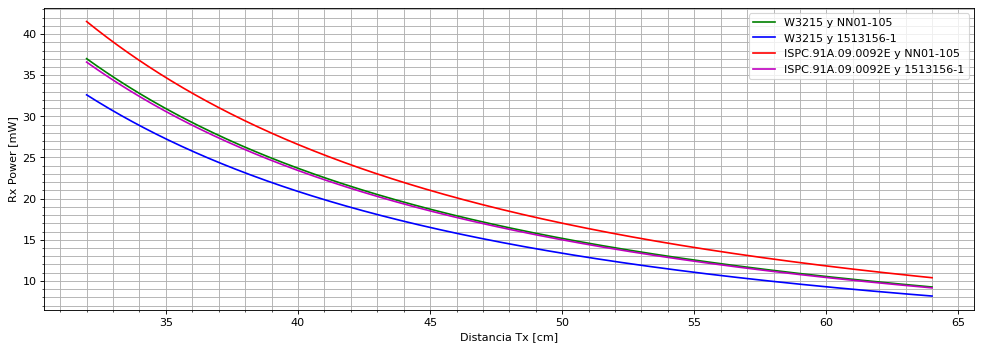
\includegraphics[width=\linewidth]{ImagenesFactibilidad/pot_recibida_teorica}
	\label{fig:pot_recibida_teorica}
	\caption{Potencia recibida en la antena Rx en función de la distancia entre antena Tx y antena Rx.}
\end{figure}

Se puede observar que con $4 \ W$ en la antena transmisora, todas las combinaciones de antenas cumplen con la potencia necesaria para el mejor y peor caso. Tomando el mejor par Rx-Tx, y al tener en cuenta la eficiencia de aproximadamente $70\%$ del P1110, la potencia a la salida de este permanece por encima del peor caso hasta la máxima distancia de transmisión.

\begin{figure}[H]
	\centering
	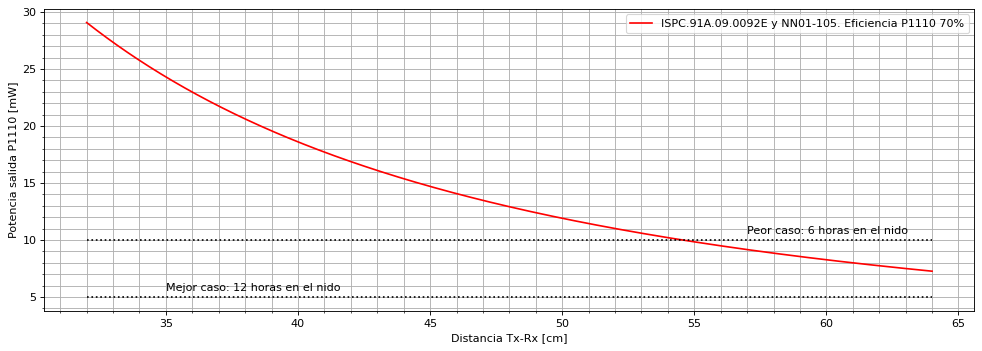
\includegraphics[width=\linewidth]{ImagenesFactibilidad/pot_baterias_teorica}
	\label{fig:pot_baterias_teorica}
	\caption{Potencia a la salida del P1110 en función de la distancia entre antena Tx y antena Rx.}
\end{figure}

Sin embargo, si se toma en consideración la restricción más estricta de $4.5 \  \frac{W}{m^2}$ impuesta en la Sección (\ref{sec:legal}) dada por la fórmula

\begin{equation}
	p = \frac{P_TG_T}{4\pi R^2}
\end{equation}

se observa en la Figura (\ref{fig:densidadradiada}) que para una potencia de $1.6 \ W$ en la antena transmisora esta restricción se cumple a treinta centímetros de la distancia mínima de transmisión.

\begin{figure}[H]
	\centering
	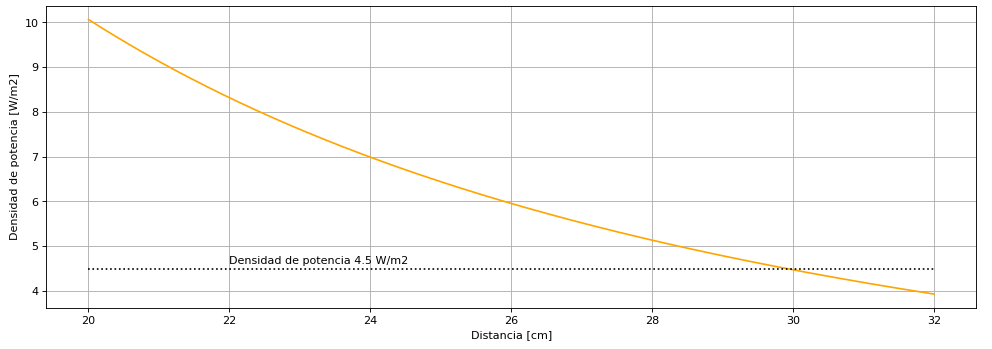
\includegraphics[width=\linewidth]{ImagenesFactibilidad/densidadradiada}
	\caption{Densidad de potencia radiada con $1.6 \ W$ en la antena transmisora según la fórmula de Friis.}
	\label{fig:densidadradiada}
\end{figure}

Teniendo esto en cuenta, y recalculando para $1.6 \ W$ se obtiene

\begin{figure}[H]
	\centering
	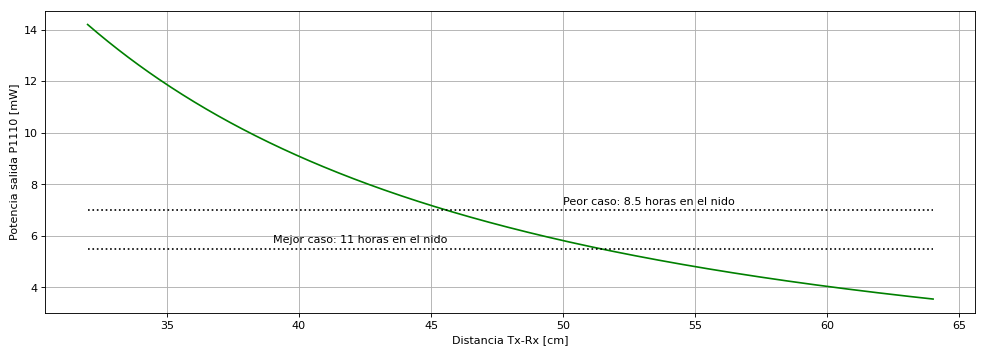
\includegraphics[width=\linewidth]{ImagenesFactibilidad/recalculo}
	\caption{Potencia a la salida del P1110 en función de la distancia entre antena Tx y antena Rx para $1.6 \ W$ en la antena transmisora.}
	\label{fig:recalculo}
\end{figure}

Por estas razones, se descarta la posibilidad de utilizar la carga inalámbrica para recargar la batería de la mochila del ave y se investigará una solución alternativa.